\section{Teorinis darbo pagrindas}

Šiame skyriuje aprašysiu teorinį darbo pagrindą.

\subsection{Mokymasis su mokytoju ir mokymasis be mokytojo}

Šiame skyriuje stengsiuosi atsakyti į klausimą kuo skiriasi mokymas su
mokytoju (angl. supervised learning) nuo mokymo be mokytojo (angl.
unsupervised learning). Mokymasis, duomenų klasifikavimo kontekste, reiškia modelių
(pvz. klasifikatorių) kūrimo metodus (algoritmus), kurie naudoja
mokymosi duomenis\footnote{Mokymosi duomenys (angl. sample data)- duomenys,
kurie yra paruošti darbui programų, kurios kurs modelius (pvz.
klasifikatorius).}, kitaip tariant, tai mokymasis iš pavyzdžių.

\subsubsection{Mokymas su mokytoju}

Mokymas su mokytoju tai toks mokymas, kai turime mokymo duomenis, kuriems jau
yra priskirtos tam tikras teisingas atsakymas. Kitaip tariant, mes sprendžiame
uždavinį, kuriam atsakymą galime pasitikrinti. Mokymas su mokytoju yra
skirstomas į dvi rūšis:
\begin{enumerate}
  \item Klasifikavimas (angl. classification) - pagal nepriklausomus
  kintamuosius bandome nuspėti kokybinius (kategorinius) priklausomus kintamuosius. 
  \item Regresija (angl. regression) - pagal nepriklausomus kintamuosius bandome
  nuspėti kiekybinius priklausomus kintamuosius.
\end{enumerate} 

%% JG: Pateik vizualų klasifikavimo pavyzdį iliustruojanti visus 3 etapus.
%% DJ: Vizualų, ta prasme su paveiksliukais ar ir tas pavyzdys su paštu
% pakankamai vaizdingas?

%% JG: Reikia kitaip struktūrizuoti šitą skyrių: 
% +Pradžioj pasakyk, kad yra klasifikavimas ir regresija ir po
%  sakinį kiekvienam.
% +Tada aptark klasifikavimą ir pateik pavyzdį. 
% +Tada pateik regresijos pavyzdį.
% +Tada parašyk, kad šiame darbe studijuojama klasifikavimo problema.

\paragraph{Klasifikavimo uždavinio pavyzdys}

Klasifikavimo tikslas - identifikuoti parametrus, kurie nusakytų grupę (klasę),
kuriai priklauso objektas. Klasifikavimo sąvoka gali būti naudojama tiek esamų
duomenų suvokimui, tiek naujų objektų charakteristikų prognozavimui.
Klasifikavimo uždavinių aktualumą galima parodyti tokiu pavyzdžiu.

\begin{figure}[htb]
\begin{center}
\leavevmode
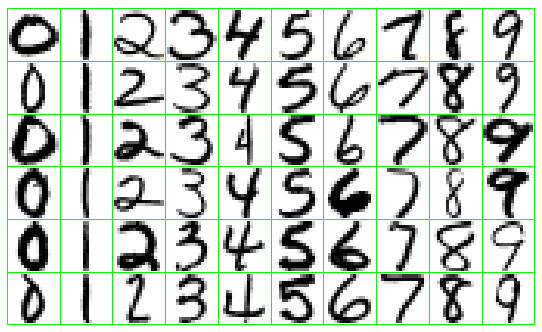
\includegraphics[width=0.5\textwidth]{images/ranka_rasyti_skaiciai.png}
\end{center}
\caption{Ranka rašytas tekstas, kurį reikia atpažinti.}
\label{fig:flash}
\end{figure}

Uždavinys: Pašto skyriuose laiškai siunčiami įvairiomis kryptimis pagal gavėjo
adresą ir (arba) pašto kodą. Norima automatizuoti laiškų rūšiavimą pagal
siuntimo kryptį. Tam, kad būtų galima laiškų rūšiavimą pagal kryptį
automatizuoti, mums reikia priemonės atpažinti ant voko užrašytą
pašto kodą.

Sprendimas: Šią problemą mums padėtų išspręsti skeneris ir programine įranga,
kuri sugebėtų ranka rašytus skaitmenis atpažinti ir konvertuoti į skaitmeninį
formatą. Tų skaitmenų atpažinimui ir konvertavimui į skaitmeninį formatą,
tikėtina, kad mes naudosime klasifikavimo algoritmus, nes uždavinys pasižymi
visomis klasifikavimui būdingomis savybėmis: turime aibę duomenų (vaizdinė
informacija su ranka rašytais skaitmenimis), turime teisingus atsakymus (žmogus
pažiūrėjęs į ranka rašytą skaitmenį gali pasakyti programai, koks ten yra
skaitmuo), bei galimų sprendimai yra kategorinio tipo (dešimt skaitmenų nuo
0 iki 9).

Klasifikatorių kursime trimis etapais:
\begin{enumerate}
  \item diskriminavimo (atskiriančiųjų) kintamųjų parinkimas - nuskenuotų
  pašto kodų skaitmenų dažniausiai pasitaikančių, charakteringiausių linijų
  radimas,
  \item klasifikavimo taisyklių sudarymas - pagal tam tikrą charakteringiausių
  linijų grupę objektui priskiriama klasė,
  \item klasifikavimo kokybės įvertinimas - kokybei įvertinti naudojami įvairūs
  metodai, tokie kaip kryžminis patikrinimas (angl. cross-validation) ir
  įkelčių metodas (angl. bootstrap).
\end{enumerate}

Įgyvendinę aukščiau aprašyto uždavinio sprendimą, pašto skyriaus vadybininkai
galėtų atlaisvinti žmones nuo iš esmės mechaninio darbo - rūšiuoti laiškus.
Tokiu būdu būtų optimizuotas pašto skyrių efektyvumas.

\paragraph{Regresinės analizės payzdys}

Regresija prognozuojant naujų duomenų reikšmes naudojasi žinomais, jau turimais
duomenimis. Ji naudoja standartinius statistinius metodus, tokius kaip mažiausių
kvadratų metodas (angl. least squares). Regresinė analizė dažniausiai naudojama
įvertinti (ang. forecast) ateities duomenų vertes bei interpoliacijai -
funkcijos tikėtinos reikšmės tarp dviejų taškų įvertinimui.

Tipinio uždavinio, kuriam naudojama regresinė analizė pavyzdys: Aktuarinėje
(draudimo) matematikoje reikia turėti įverčius, pasakančius kokia tikimybė, kad
žmogus vienokio ar kitokio amžiaus mirs. Tam yra naudojamos taip vadinamos 
mirtingumo lentelės. Jose duomenys aprašo kiek ir kokio amžiaus žmonių
kažkuriais metais mirė, pvz. 2010 metais Lietuvoje mirė 1000 20 metų amžiaus 
žmonių. Detalesni duomenys nėra naudojami, nes per daug sudėtinga juos apdoroti.
Kadangi aktuarai nori apskaičiuoti draudimo kainą, jiems reikia įvertinti
riziką, kada žmogus mirs, tai jie naudodamiesi regresinės analizės metodais 
paskaičiuoja tikėtiniausią reikšmę, kad pvz. yra 3\% tikimybė, kad žmogus  mirs
dvidešimtaisiais savo gyvenimo metais. Kitais žodžiais tariant, iš turimų
duomenų mes sukursime tolydžią funkcija, kuri mums pasakys reikšmes taškuose,
kurių mes neturime.

\paragraph{Klasifikavimas ir regresija}

Abiejų mokymo su mokytoju rūšių tikslas yra pagal mokymosi duomenis sukurti
modelį, kuriuo remiantis būtų galima identifikuoti naujų objektų
savybes.\cite{markhall99} Šiame darbe negrinėsime klasifikavimo problemą.

\subsubsection{Mokymas be mokytojo}

Mokyme su mokytoju galima išmatuoti modelio tikslumą įvairiais metodais, pvz.
kryžminiu patikrinimu. Mokyme be mokytojo mes tokių tiesioginio patikrinimo
procedūrų neturime. Todėl yra sunku išsiaiškinti patikimumą išvadų gautų pagal
daugumos mokymo be mokytojo algoritmų darbo rezultatus. 

Klasterizavimo algoritmų pagrindinis privalumas – gebėjimas atpažinti grupavimo
struktūrą be jokios išankstinės informacijos. 

Klasterizavimo principas - maksimizuoti objektų, esančių vienoje grupėje,
tarpusavio panašumą ir minimizuoti tarpgrupinį objektų panašumą.


<<<<<<< HEAD
=======
{\centering>>>>Pritrūkau sveikatos šįvakar pribaigti tą skyrių. <<<< }

>>>>>>> a2900dcdfd177b5ce954f7c78becbe2337abbb07
%% JG: neprižiūrimų mokymosi metodų yra visokių: association rule mining,
% clustering, ir t.t. Zr ESL knygos 14 skyrių.
%% DJ: Nurašinėjau nuo Duda knygos tą vietą, kur mokymas be mokytojo ir 
% klasterizavimas yra sinonimai.

%% Kartais šiokia tokia informacija žinoma. Pvz., klasterių kiekis nurodomas
% k-means algoritme. Arba galima daryti prielaidas apie klasterių struktūrą:
% k-means ieško apvalių klasterių. Esminis dalykas yra tas, kad teisingas
% atsakymas nėra žinomas.

%% JG: algoritmas turi atrasti grupes duomenyse, jos nėra iš anksto žinomos.

\subsubsection{Mokymo su mokytoju ir mokymo be mokytojo skirtumai}

Pagrindiniai skirtumai tarp mokymo su mokytoju ir mokymo be mokytojo yra
mokymosi duomenys (mokymo su mokytoju algoritmų įeities duomenyse yra
išreikštinai pasakyta, kokio rezultato mes laukiame, o neprižiūrimojo mokymosi
duomenyse tokios papildomos informacijos nėra) ir naudojimo tikslai (mokymas
su mokytoju siekia iš pavyzdžių išmokti vertinti naujus duomenis, o mokymas be
mokytojo siekia surasti vidinę duomenų struktūras). Aptarkime pavyzdį: darbas
su nuotraukomis.

Mokymo su mokytoju programai kaip įeities duomenis paduotume keletą 
nuotraukų su žymėmis pasakančiomis, ar nuotraukoje yra žmogaus veidas ar jo ten
nėra, kitaip tariant, duotume keletą pavyzdžių su teisingais atsakymais.
Programa peržvelgs visas nuotraukas ir susikurs klasifikatorių (modelį), kuris
kažkokiu tikslumu galės atskirti nuotraukas su žmogaus veidu. Tokiu būdu mūsų
mokymo programa ,,išmoks`` nuotraukose atpažinti veidus.

Mokymosi be mokytojo programai kaip įeities duomenis paduotume keletą
nuotraukų be jokių papildomų žymių. Žinoma, mūsų programa pati nesugebės
,,išrasti``, kas yra žmogaus veidas, tačiau ji tikriausiai sugrupuos nuotraukas
su žmonių veidais ir tarkim peizažais į skirtingas grupes. Kitaip tariant,
nuotraukų su žmonių veidais vidinė struktūra mūsų mokymo be mokytojo programai
bus nepanaši nuotraukų su peizažais vidinę struktūrą, todėl ji į vieną klasterį
susidės nuotraukas, kurios jai atrodo tarpusavyje panašiausios: viename
klasteryje nuotraukos su žmonių veidais, o kitoje su gamtos peizažais.

Abu mokymo procesai yra panašūs savo esme (siekia išgauti žinias apie turimus
duomenis), bet jų panaudojimas skiriasi iš esmės (mokymo su mokytoju atveju mes
kuriame modelį apibūdinantį kaip buvo sukurti mokymo duomenys, kad galėtume
spėti naujų objektų savybes, o mokymo be mokytojo atveju siekiame susipažinti
su vidine mokymo duomenų struktūra, kai nėra kaip pamatuoti ar geri ar blogi
klasteriai buvo rasti).

%% JG: aš nesutinku, kad abiem procesais siekiama tų pačių tikslų. Vienu atveju 
% siekiama išmokti iš pavyzdžių. Kitu atveju siekiama atrasti nežinomas
% struktūras turimuose duomenyse. Procesai yra panašūs savo esme, bet jų 
% panaudojimas skiriasi iš esmės.

%% JG: iš vikipedijos: In machine learning, unsupervised learning refers to the 
% problem of trying to find hidden structure in unlabeled data. Since the
% examples given to the learner are unlabeled, there is no error or reward
% signal to evaluate a potential solution. This distinguishes unsupervised 
% learning from supervised learning and reinforcement learning.

%% JG: visą šitą skyrių reikia pateikti koncentruotai. Esminiai teiginiai ir grafiniai pavyzdžiai. 

%% DJ: Turiu pripažint, kad šitam pavyzdyje prigrybavau stipriai. Nurašinėjau
% pavyzdį kur prastai paaiškino skirtumą, bet užtat man pavyzdys patiko. Dabar
% labiau į temą surašyta.
